\documentclass{article}

\usepackage{fullpage}
\usepackage{graphicx}
\usepackage{color}
\usepackage{fancyhdr}
\usepackage{url}
\usepackage{amsmath,bm}
\usepackage{amssymb}
\usepackage{amsthm}
\usepackage{amsfonts}
\usepackage[round]{natbib}
\usepackage{enumitem,xcolor}
\usepackage[multiple]{footmisc}

\graphicspath{ {figures/} }

\usepackage[
    pdftitle={Capstone Proposal - Udacity Machine Learning Nanodegree},
    pdfsubject={Machine Learning, Reinforcement Learning, Deep Learning, Artificial Intelligence, Games},
    pdfauthor={David Robles},
    pdfpagemode=UseOutlines,
    pdfborder= {0 0 1.0},
    bookmarks,
    bookmarksopen,
    colorlinks=true,
    citecolor=blue,
    linkcolor=blue, %
    linkbordercolor=blue, %
    urlcolor=blue, %
]{hyperref}

\usepackage[labelfont=bf]{caption}


\usepackage[utf8]{inputenc}

% Default fixed font does not support bold face
\DeclareFixedFont{\ttb}{T1}{txtt}{bx}{n}{8} % for bold
\DeclareFixedFont{\ttm}{T1}{txtt}{m}{n}{8}  % for normal

% Custom colors
\usepackage{color}
\definecolor{deepblue}{rgb}{0,0,0.5}
\definecolor{deepred}{rgb}{0.6,0,0}
\definecolor{deepgreen}{rgb}{0,0.5,0}

\usepackage{listings}

\definecolor{codebg}{RGB}{238,238,238}

% Python style for highlighting
\newcommand\pythonstyle{\lstset{
language=Python,
basicstyle=\ttm,
otherkeywords={self},             % Add keywords here
keywordstyle=\ttb\color{deepblue},
emph={MyClass,__init__},          % Custom highlighting
emphstyle=\ttb\color{deepred},    % Custom highlighting style
stringstyle=\color{deepgreen},
frame=tb,                         % Any extra options here
framesep=10pt,
framexleftmargin=10pt,
backgroundcolor=\color{codebg},
rulecolor=\color{codebg},
aboveskip=10pt,
belowskip=10pt,
showstringspaces=true            %
}}


% Python environment
\lstnewenvironment{python}[1][]
{
\pythonstyle
\lstset{#1}
}
{}

% Python for external files
\newcommand\pythonexternal[2][]{{
\pythonstyle
\lstinputlisting[#1]{#2}}}

% Python for inline
\newcommand\pythoninline[1]{{\pythonstyle\lstinline!#1!}}



%%%%%%%%%%%%%%%%%%%%%%%%%%%%%%%%%%%%%%%%%%%%%%%%%%%%%%%%%%%%%%%%%%%%%%%%%%%%%%%%%%%%%%%%%%%%%%%%%%%%
\title{Machine Learning Nanodegree \\ Toxic Comment Text Classification Challenge}
\author{Sam Mottahedi}
\date{01/08/2018}
\begin{document}
\maketitle


\section{Definition}

    \subsection{Project Overview}

    Natural language processing (NLP) is one of the most important technologies of the information age. Understanding complex language utterances is also a crucial part of artificial intelligence. Applications of NLP are everywhere because people communicate most everything in language: web search, advertisement, emails, customer service, language translation, radiology reports, etc. There are a large variety of underlying tasks and machine learning models behind NLP applications.


    \subsection{Problem Statement}


    Free expression and sharing information is the greatest impact of internet in modern society. Unfortunately, online abuse and harassment can lead limit self expression on the web. Many platforms struggle to effectively
    facilitate conversations, leading many communities to limit or
    completely shut down user comments.

    In this \href{https://www.kaggle.com/c/jigsaw-toxic-comment-classification-challenge}{Kaggle competition} ,  participant are challenged to build a multi-headed model that’s capable of detecting different types of of toxicity like threats, obscenity,insults, and identity-based hate.In order to accomplish this objective, a Recurrent Neural Network (RNN) Architecture with Gated Recurrent Units (GRU) were used which are suitable for processing information in the form of sequence of words. An Attention Mechanism is used in order to improve the performance of the model by focusing on important parts of input sequence. Multi-Task learning objective is added to network to improve the generalization error and reduce over-fitting to the training data set.



    \subsection{Metrics}

    Submissions are evaluated on the mean column-wise log loss. In other words, the score is the average of the log loss of each predicted column.


    Since class labels are not mutually exclusive, a multi-label classification loss function is required here. Multi-label classification (MLC) is a prediction problem in which several class labels are assigned to single instances simultaneously as follows:

    \begin{equation}
            loss(\hat{y}, y) = \frac{1}{|L|} \sum_{l=1}^{l=|L|} - (y_l - log(\hat{y_l}) + (1-y_l) \cdot log(1-\hat{y_l}))
    \end{equation}



\section{Analysis}

    \subsection{Data Exploration}

    The \href{https://www.kaggle.com/c/jigsaw-toxic-comment-classification-challenge/data}{Kaggle competition dataset} provided is Wikipedia Human Annotations of Toxicity on Talk Pages and contains $160,000$ human labelled annotations based on asking 5000 crowd-workers to rate Wikipedia comments according to their toxicity (likely to make others leave the conversation). Each comment was rated by 10 crowd-workers. The Test dataset which is used to evaluating performance in competition consist of $226,998$ unlabeled comments. Each comment in the training set can be labeled with $6$ labels which are not mutually exclusive.

    The toxic comment data set have the following fields:

    \begin{itemize}
        \item "id": (string)
        \item "comment texts": comments (string)
        \item "toxic": toxic comment label (binary)
        \item "sever toxic": severely toxic comment label (binary)
        \item "obscene": obscene comment label (binary)
        \item "threat": threatening comment label (binary)
        \item "insult": insulting comment label (binary)
        \item "identity hate": identity hate comment label (binary)
    \end{itemize}

            % These 6 labels wit their prevalence are:

        % \begin{itemize}
        %         \item Toxic ($0.4300$)
        %         \item Severe Toxic ($0.0455$)
        %         \item Obscene ($0.2410$)
        %         \item Threat ($0.0144$)
        %         \item Insult ($0.2248$)
        %         \item Identity hate ($0.0384$)
        % \end{itemize}


    \subsection{Exploratory Visualization}

    It is important to know how labeled comment are distributed in the dataset and wether or not they the labels as balanced. Figure \ref{fig:labels} shows the distribution of labels

    \begin{figure}[!h]
        \centering
        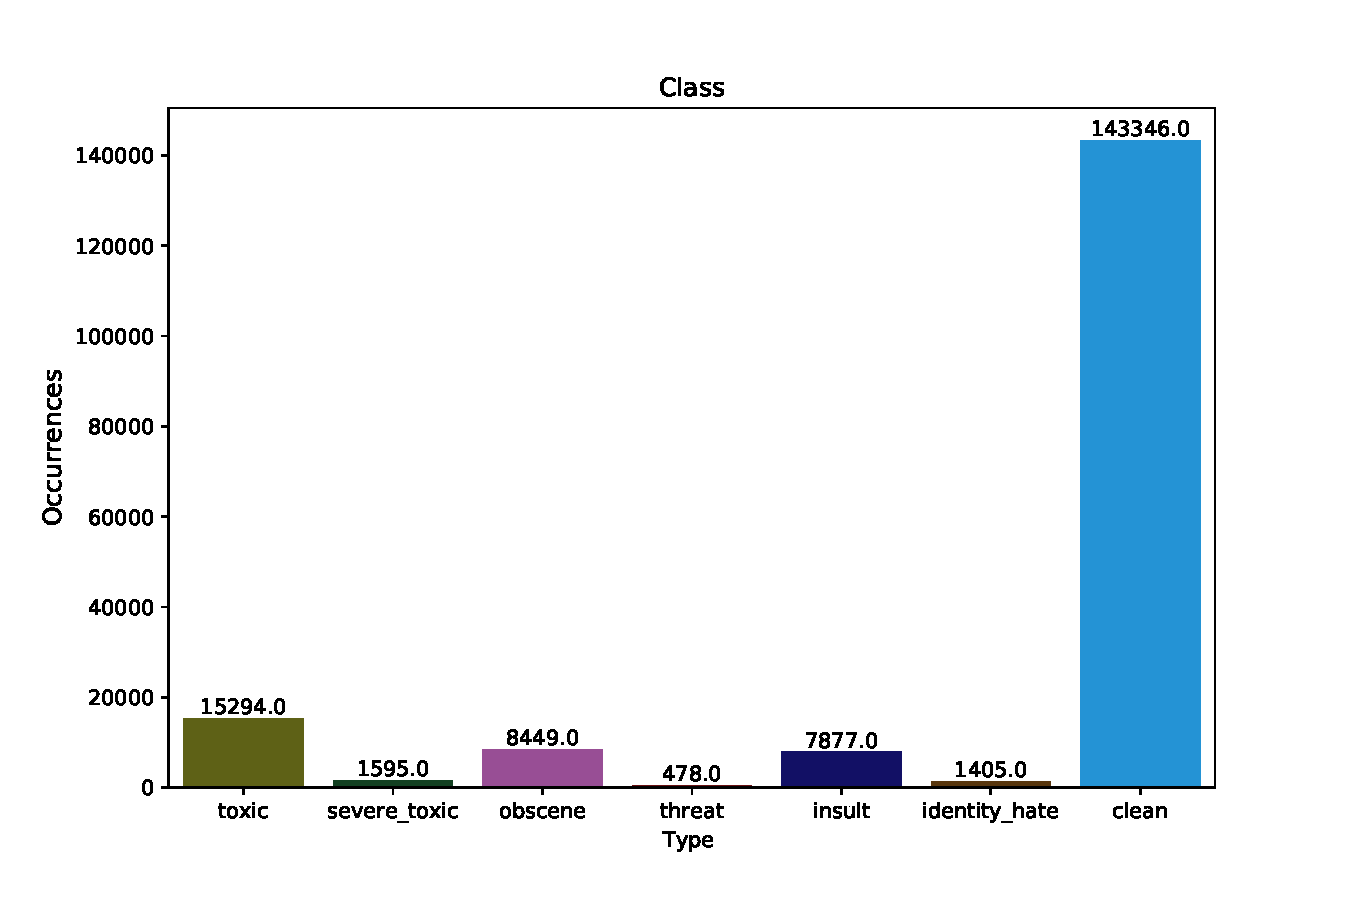
\includegraphics[scale=0.7]{figures/labels.pdf}
        \caption{Toxic comment dataset label distribution}
        \label{fig:labels}
    \end{figure}

    The plot shows that most of the comments are innocent and small number of comments are classified as any form toxic comment. The comments classified as severely toxic, threat and identity hate are rare compared to toxic, obscene and insult.

    An example of a comment is provided bellow with was labeled as both toxic and a threat.

    \begin{verbatim}
        ('Hi! I am back again!\nLast warning!\nStop undoing my edits or die!',
    \end{verbatim}

    As it can be seen, the comments are not clean and contain many signs, symbols and spelling errors that makes the classification problem based on word level vectors much harder.

    It's also helpful to look at word could of comments labeled with any of toxic comments labels (Figure \ref{fig:wordcloud}):

    \begin{figure}[!h]
        \centering
        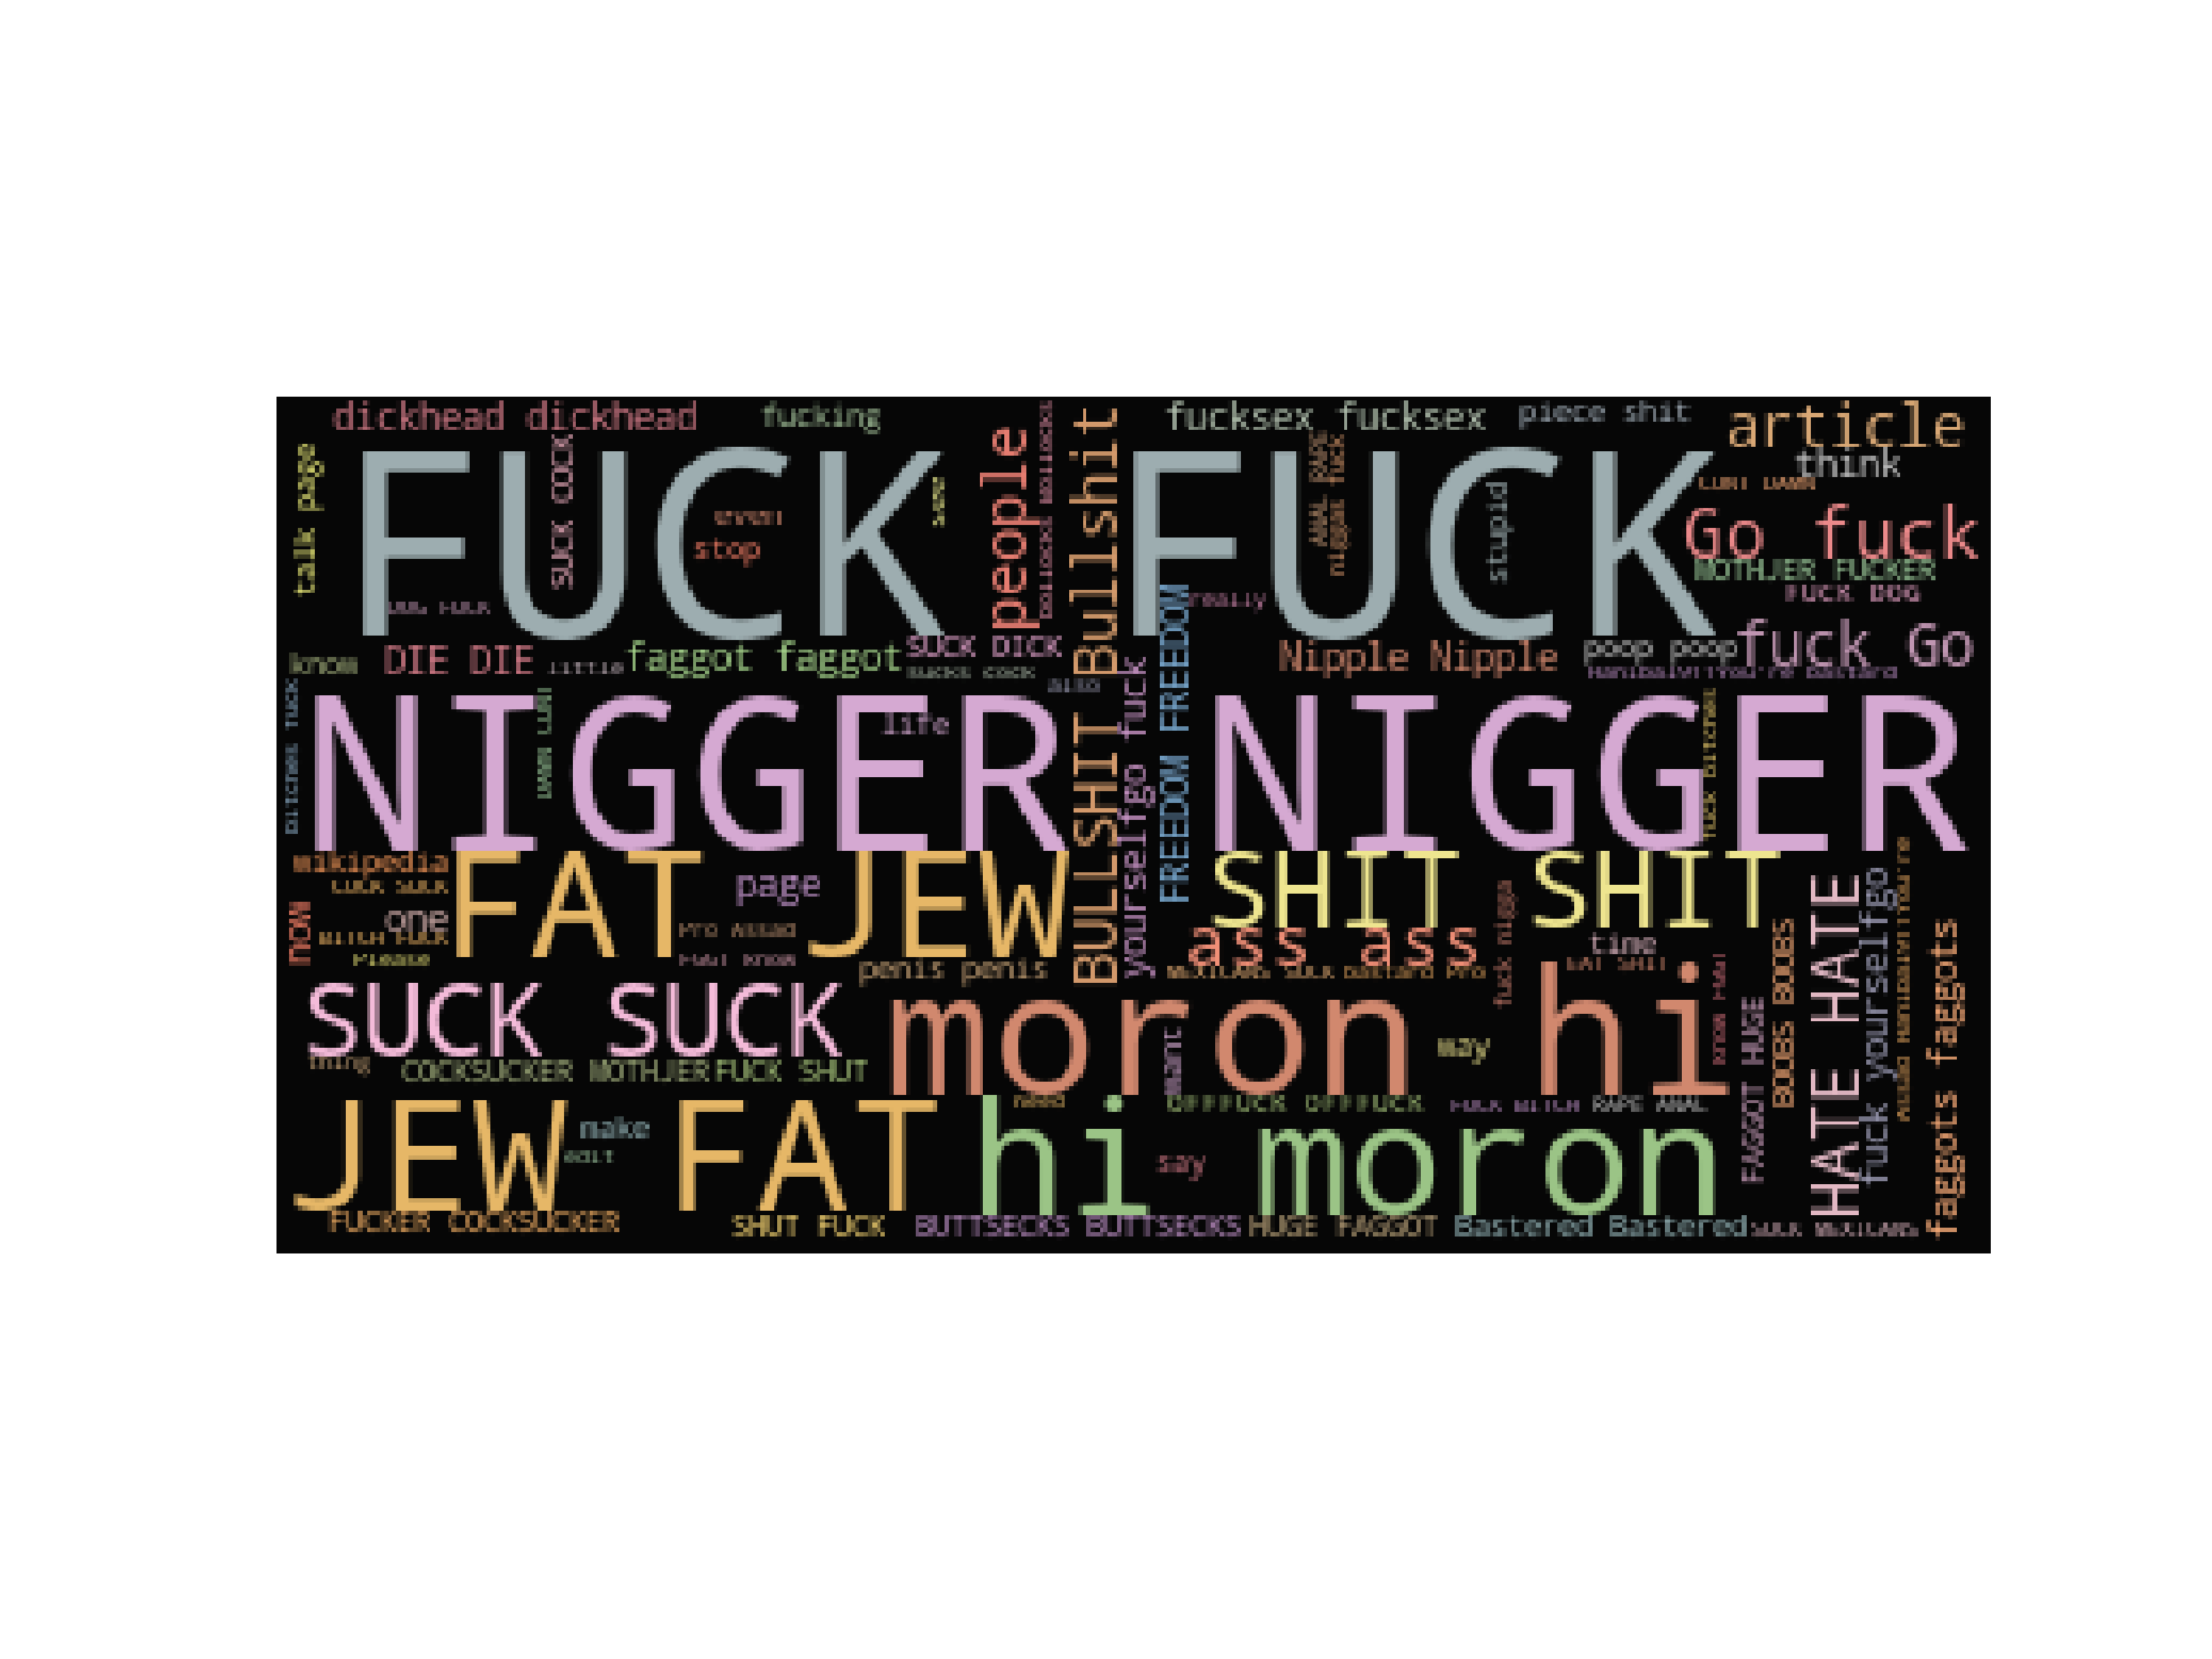
\includegraphics[scale=0.3]{figures/wordcloud.pdf}
        \caption{Toxic Comment WordCloud}
        \label{fig:wordcloud}
    \end{figure}


    The data will be divided in to 3:1:1 for training validation and testing. Since the labels are not balanced, during the training each batch of data will be sampled using a Stratified sampling method to expose the model to different class labels.

    \subsection{Algorithms and Techniques}

    Recurrent neural network architectures combining with attention mechanism,
    or neural attention model, have shown promising performance recently for
    the tasks including speech recognition, image caption generation,
    visual question answering and machine translation.
    In the sequence labeling tasks,
    the model input is a sequence, and the output is the label of the
    input sequence. The major difficulty of sequence labeling is that when
    the input sequence is long, it can include many noisy or irrelevant parts.
    If the information in the whole sequence is treated equally, the noisy or
    irrelevant part may degrade the classification performance.
    The attention mechanism is helpful for sequence classification task because
    it is capable of highlighting important part among the entire sequence for
    the classification task.

    Recurrent neural networks (RNNs) are class of neural networks designed for processing sequential data [\cite{goodfellow2016deep}]. Compared to feed forward neural networks, RNNs are able to scale to longer sequences which in most part is not practical without sequence-based networks. Generally, RNN are implemented by unrolling the computational graph and sharing wmodel parameters across deep network structure. RNNs are trained using Back-Propagation Through Time (BPTT) which is variation of ordinary back-propagation applied to an unrolled computational graph. Deep RNNs usually face complication due to Long-Term dependencies [\cite{goodfellow2016deep}] such as vanishing and exploding gradients. Most effective solution to overcome these problem is the use of Gated Recurrent Units (GRUs) which is based on idea of creating pathways through time that have derivatives that neither vanish nor explode. GRUs accomplish this by introducing self loops to add pathways were gradient can flow for long duration.


    In this project, each comment is treated as set of features using pre-trained GloVe word embedding. A Bi-directional recurrent neural network with Gated Recurrent Units (GRU). Attention mechanism is added on top of the Bi-directional RNN which improve the performance of the model focusing on important parts of long sequence and reduce the effect of noise and unrelated information. The classification task is a multi-label classification where comments toxicity labels are not mutually exclusive.



    \subsection{Benchmark}

    The baseline chosen here in order to get better understanding of the problem from a general machine-learning perspective. To this end, the baseline model is chosen to be a logistic regression model based on Term Frequency-inverse document frequency data which can achieve column-wise log-loss of $0.05567$.



\section{Methodology}

    \subsection{Data Processing}

    The preprocessing is mostly done using functions available in data.py module. The preprocessing step  before training or testing consist of following steps:

    \begin{itemize}
        \item Preprocessing comments:
            \begin{itemize}
                \item tokenizing
                \item converting to lower-case letters
                \item removing stopwords
                \item normalizing numbers, date, ...
            \end{itemize}

        \item Vocabulary: creating dictionary of words with at least $count() > Thresh_hold$.
        \item Index to word: dictionary with keys equal to word index and values being a word in the vocabulary
        \item Word to index: dictionary with keys equal to vocabulary's word and value being words index.
        \item Sequence index file: a file containing sequence of word index for each comment.
    \end{itemize}

    During training, the pre-processed comment are read from sequence to index file and push to TensorFlow input placeholders. In addition, at the beginning of the training the word vectors corresponding to the words in the vocabulary are extracted from pre-trained GloVE word vector with $6$ Billion words and specified word vector dimension.

    The preprocessing process has the following adjustable parameters:

    \begin{itemize}
        \item Word frequency threshold
        \item GLoVe word vector dimension (50, 100, 200)
        \item Using trainable or not trainable word vector tensor
        \item Maximum input sequence length
    \end{itemize}



    \subsection{Implementation}

    \subsubsection{Text Classification with Recurrent Neural Networks}

    The architecure used in this work is Recurrent Neural Network (RRN) that takes the sequence of words index and an encode the information in the text in the last output layer. First we need to lookup word-vectors corresponding to each word in the input sequence. The embedding matrix and the embedding lookup operation defined using TensorFlow as:

    \begin{python}
    @lazy_property
    def _create_embedding(self):
        with tf.name_scope('Embeddings'):
            if self.pre_train:
                self.embedding = tf.Variable(tf.constant(0.0,
                                                        shape=[config.VOCAB_SIZE,
                                                        config.GLOVE_SIZE]),
                                                        trainable=config.TRAINABLE_EMBEDDING)
                self.embedding_init = self.embedding.assign(self._embedding_placeholder)

            else:
                self.embedding = tf.Variable(tf.random_uniform(
                    [config.VOCAB_SIZE, config.EMBEDDING_DIMENSION], -1.0, 1.0))
    embed = tf.nn.embedding_lookup(self.embedding, self._inputs)
    \end{python}

    Since some of the comments are quite long, a Bi-directional RNN is used which has two Gated Recurrent Cells (GRU) for forward and backward processing of the input sequence and outputs the concatenated output oof the forward and backward cell [figure \ref{figure:bi-rnn}].     The GRU forward and backward cell are and the bi-directional dynamic RNN are defined in the \pythoninline{_inference} method of \pythoninline{SeqClassifier} class:

    \begin{figure}
        \centering
        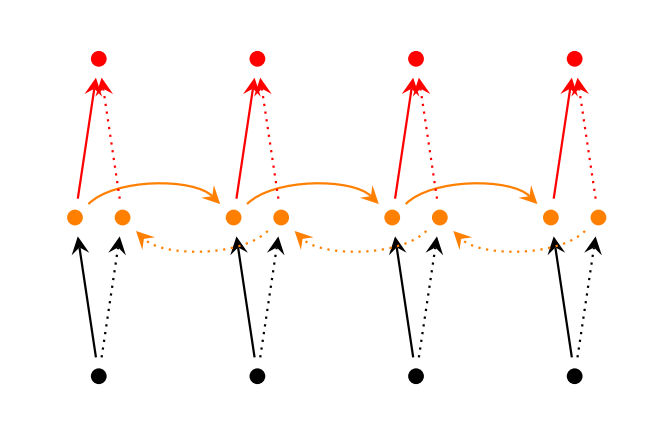
\includegraphics[scale=0.6]{bi_rnn.png}
        \caption{Bi-directional RNNs}
        \label{figure:bi-rnn}
    \end{figure}



    \begin{python}
    with tf.name_scope('Bi-GRU'):
    with tf.variable_scope('forward'):
        gru_fw_cell = tf.contrib.rnn.GRUCell(
            config.HIDDEN_LAYER_SIZE)
        if self.mode == 'train':
            gru_fw_cell = tf.contrib.rnn.DropoutWrapper(gru_fw_cell,
            output_keep_prob=config.KEEP_PROB )

    with tf.variable_scope('backward'):
        gru_bw_cell = tf.contrib.rnn.GRUCell(
            config.HIDDEN_LAYER_SIZE)
        if self.mode == 'train':
            gru_bw_cell = tf.contrib.rnn.DropoutWrapper(gru_bw_cell,
            output_keep_prob=config.KEEP_PROB)

        outputs, states = tf.nn.bidirectional_dynamic_rnn(cell_fw=gru_fw_cell,
                                                    cell_bw=gru_bw_cell,
                                                    inputs=embed,
                                                    sequence_length=self._seq_length,
                                                    dtype=tf.float32,
                                                    scope='Bi-GRU')
    states = tf.concat(values=states, axis=1)
    \end{python}

    It is important to note that the Dropout should only apply at the time of training. The last output layer of the RNN is concatenated and passed through two feed forward layers and a final layer with $6$ output nodes where a element wise sigmoid function is applied and a multi-label predictions are generated.


    \subsubsection{Attention Mechanism}
    Since not all words contribute equally to the representation of the sequence meaning we need to use an attention mechanism [\cite{yang2016hierarchical}] that extract important words to the meaning of the sequence and aggregates the presentation of informative words to form a sentence vector from [figure \ref{fig:attention}

    \begin{align}
        u_{it} = tanh(W_w h_{it} + b_w) \\
        \alpha_{it} = \frac{exp(u_{it}^T u_w)}{\sum_t exp(u_{it}^T u_w)} \\
        o = \sum_t \alpha_{it}h_{it}
    \end{align}

    where the word annotation $h_{it}$ is passed to a one-layer MLP to get $u_it$ as hidden representation $h_it$  the importance of the word is measured by comparing $u_{it}$ to a word context vector $u_w$ and then passed through a softmax function to get normalized importance weight $\alpha_{it}$ and the output vector is weighted sum of word annotation based of the weights. The context vector is randomly initialized and jointly learned during the training process.

    \begin{figure}
        \centering
        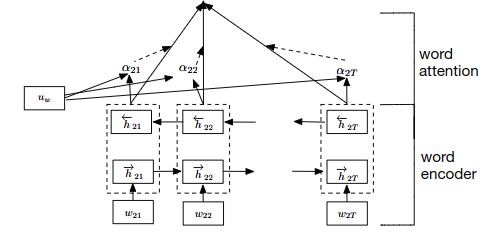
\includegraphics[scale=0.7]{attention.png}
        \caption{Attention Mechanism \cite{yang2016hierarchical}}
        \label{fig:attention}
    \end{figure}

    \begin{figure}
        \centering
        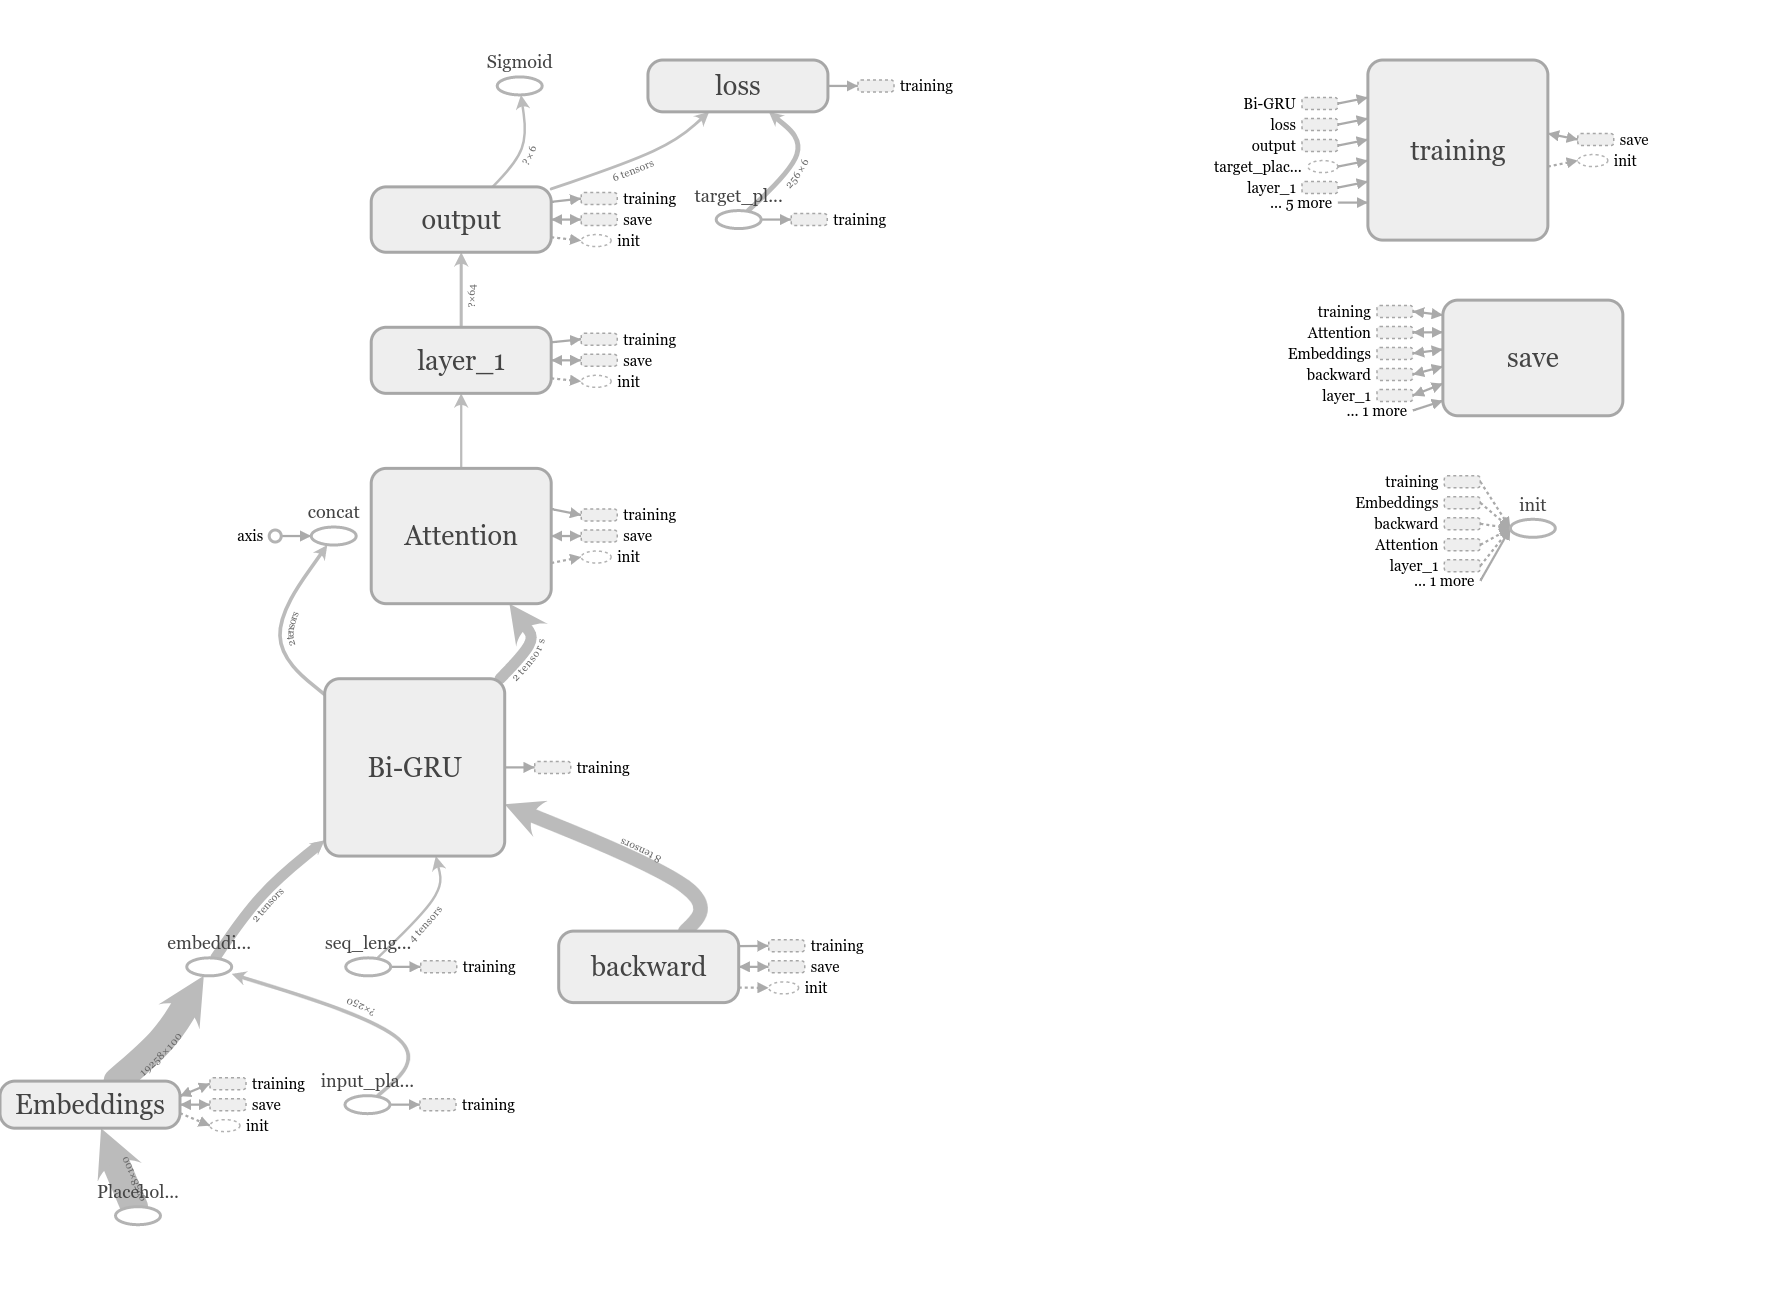
\includegraphics[scale=0.3]{tensorflow.png}
        \caption{TensorFlow computational graph for sequence classification model with attention mechanism}
        \label{fig:tensorflow}
    \end{figure}


    The optimizer used here is Stochastic Gradient Decent with exponentially decaying learning rate defined as:

    \begin{python}
    def _create_optimizer(self):
    with tf.variable_scope('training') as scope:
        self.global_step = tf.Variable(0, dtype=tf.int32, trainable=False,
                                        name='global_step')

        if self.mode == 'train':
            with tf.name_scope('learning_rate'):
                self.learning_rate = tf.train.exponential_decay(config.LR, self.global_step,
                                        10000, 0.96, staircase=True)
                tf.summary.scalar('learning_rate', self.learning_rate)
            self.optimizer = tf.train.GradientDescentOptimizer(self.learning_rate)
            trainbales = tf.trainable_variables()
            start = time.time()
            clipped_grads, self.gradient_norms = tf.clip_by_global_norm(tf.gradients(self.losses,
            trainbales), config.MAX_GRAD_NORM)
            self.train_ops = self.optimizer.apply_gradients(zip(clipped_grads, trainbales),
            global_step=self.global_step)
            print('creating opt took {} seconds'.format(time.time() - start)
    \end{python}

    It can be seen that the gradient are manually applied and the gradient norm is clipped at $1$ to prevent problems due to exploding gradients. The completed TensorFlow computational graph can be seen in Figure [\ref{fig:tensorflow}]

    \subsection{Refinement}

    \subsubsection{Multi-Task Learning}
        In order to prevent over-fitting to training set and auxiliary loss was added to the computational graph. \cite{caruana1998multitask} showed that multi-task learning improves generalization by leveraging the domain-specific information contained in the training signal of related task. Here, the auxiliary task used is the log-loss error for predicting if any form of comment toxicity is observed. Since large number of comments didn't classified as toxic comment, this auxiliary task help better discriminating toxic comments. The scheme used here is Hard Parameter Sharing \cite{caruanamultitask}, which the parameters are shared between all task while keeping several task-specific output layers (Figure \ref{fig:mtl}).

        \begin{figure}
            \centering
            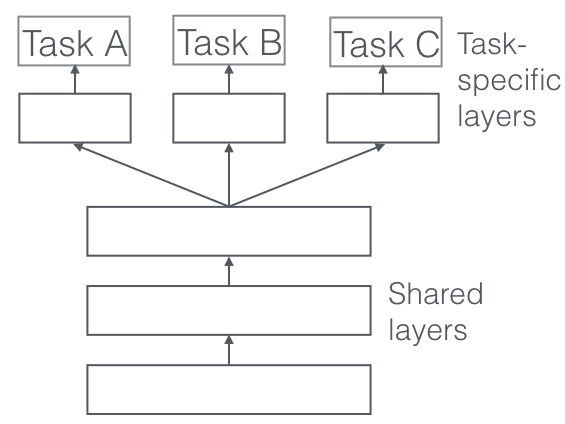
\includegraphics[scale=0.4]{mtl.png}
            \caption{Multi-task learnng with Hard Parameter Sharing.}
            \label{fig:mtl}
        \end{figure}

        Addition of multi-task layer resulted in $17\%$ reduction in validation log-loss value from $0.04123$ to $0.0342$.

\section{Results}

    \subsection{Model Evaluation and Validation}

    During development process, the training data was split into training ($90\%$) and validation ($10\%$) sets. Since this project is part of Kaggle competition, instead of using a test set the submission result is used as a metric for final evaluation of the model.

    The final description of the final model is as follows:


    \begin{itemize}
        \item Batch Size = 256
        \item Embedding dimension = 100
        \item Number of GRU Cells = 128
        \item Feed-forward layers = 128
        \item Attention size = 256
        \item Maximum input sequence length = 250
    \end{itemize}

    An early-stopping mechanism is implemented to automatically save model weights corresponding to best evaluation log-loss and stop the training to prevent over-fitting to the training set. The best results obtained from a single model with attention mechanism and multi-task loss objective are 0.0281 log-loss on the training set and 0.0342 on the validation set. The best score obtained on the test dataset by submitting the prediction on Kaggle competition is 0.0362 log-loss. Recently the competition has change the metric form column-wise log-loss to column-wise Receiver Operator Characteristic Area Under the Curve (ROC AUC). The score obtained using the new evaluation metric is 0.9440.


    \subsection{Justification}

    Using the RNN based text classification with attention mechanism and the lowest log-loss error achieved is 0.0342 which shows a $38.56\%$ reduction compared to log-loss error obtained using the benchmark model. The reduction in error is significant and justifies the computational cost of training a deep architecture.


\section{Conclusion}


    \subsection{Free-Form Visualization}

    In order to visual the significance of solution used for this specific problem, attention layer weights and the increase importance of words in the input with higher attention weights is provided in Figure \ref{fig:att_image}. It can be seen that model learned to pay more attention to words that contain profanities.

    \begin{figure}
        \centering
        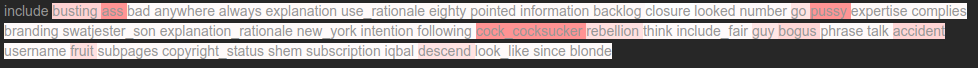
\includegraphics[width=7in, height=1in]{att_image.png}
        \caption{Attention layer Visualization}
        \label{fig:att_image}
    \end{figure}



    \subsection{Reflection}

    In this project a deep recurrent neural network was trained to predict if the input text includes multiple profanity or contains content that and can negatively effect the online community. Since the text in the comments include many non-standard form form of speech or incorrect spellings, significant effort was required for preprocessing the text. Since in most cases, the observed comments were long, a recurrent neural neural network with attention mechanics was implemented that is immune to common problem in these situation such as vanishing gradient, exploding gradient and etc. The proposed model was compared to a logistic1 regression model based on tf-idf data which shows significant reduction in log-loss error and justifies the additional computational cost.


    \subsection{Improvement}
    This project can use improvements in many respects, First, larger model with many additional hidden layers can improve the generalization and result in better prediction. Also, more training data can certainly improve the results. Other measures such as pre-training on similar data set can alo improve the generalization. In addition, like many Kaggle competition the best results are based on ensemble of many models and is possible solution to improve the predictions.


\bibliographystyle{plainnat}
\bibliography{bibliography.bib}

\end{document}